\section{Resource Sharing and Binding Analysis}

As explain before two or more operation can be bound to the same resource. Before we bond them together we need to ensure that they are \textit{compatible}. Two conditions that the operations should met in order to be \textit{compatible} :

\begin{itemize}
\item The operations is not concurrent.
\item The operations can be implemented by resources of the same type.
\end{itemize}

So, $ E+\{(v_{i},v_{j})|\tau(v_{i}=v_{j} $ and $ ((t_{i}=d_{i} \leq t_{j}) $ or $ t_{j}=d{j} \leq t_{i})),i,j=1,...,n_{ops}\}$ %

In general, the compatibility can be analyzed using compatibility graph, conflict graph. The sample problem that I will use for the explanation is from figure \ref{fig:Scheduled_sequencing_graph}


\subsection{Compatibility Graph}


$G_{+}(V,E)$ is a graph whose vertex set  $  V = \{v_{i}, i = 1,2,..., n_{ops}\} $ is in one to one correspondence with the operation and whose edge set $ E = \{\{v_{i},v_{j} i,j = 1,2,...,n_{ops}\}$ denotes the compatible operation pairs \cite{b1}. 

Means that the number of disjoint component in the graph has atleast the same number with the resource types. An optimum resources sharing is one that minimizes the number of required resources instance \cite{b1}.

According to \cite{b1} - A group of mutually compatible operations corresponds to a subset of vertices that are all mutually connected by edges, i.e., to a clique. Therefore a minimal set of mutually compatible operations is represented by a maximal clique in the compatibility graph. Since we can associate a resource instance to each clique, the problem is equivalent to partitioning the graph into a minimum number of cliques. Such a number is the clique cover number of $G_{+}(V,E)  $, denoted by $\kappa(G_{+}(V,E)) $

Figure \ref{fig:Compatibility_graph} is an example of compatibility graph base on sequencing graph in figure\ref{Scheduled_sequencing_graph}. We can see that $\{v_{2},v_{6}\}  $ and $\{v_{10},v_{11}\} $ are examples of compatible operation.  Examples of cliques are the subgraphs induced by $\{v_{1},v_{3},v_{7}\}  $,$\{ v_{2},v_{6},v_{8}\} $,$\{ v_{4},v_{5}, v_{10}, v_{11}\}$ $ \{v_{9}\} $. So the clique cover number $ \kappa $ of the graph is 4, corresponding to two multipliers and two ALUs. Edges of the cliques are emboldened in Figure \ref{fig:Compatibility_graph}.


\ref{fig:Compatibility_graph}
\begin{figure}[h]
    \centering
    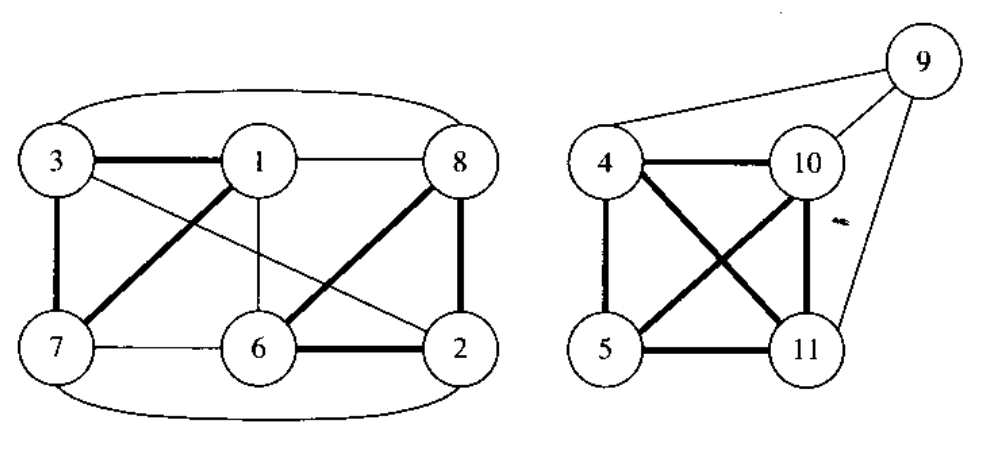
\includegraphics[width=0.5\textwidth]{Compatibility_graph}
    \caption{ Compatibility graph \cite{b1}}
    \label{fig:Compatibility_graph}
\end{figure}


\subsection{Conflict Graph}
$G_{-}(V,E)  $,  is a graph whose vertex set $  V = \{v_{i}, i = 1,2,..., n_{ops}\} $ is in one-to-one correspondence with the operations and whose edge set $ E = \{\{v_{i},v_{j} i,j = 1,2,...,n_{ops}\}$ denotes the conflicting operation pairs \cite{b1}. 

$G_{-}(V,E) $ is the compliment of $G_{+}(V,E)  $ because A set of mutually compatible operations corresponds to a subset of vertices that are not connected by edges, also called the independent set $G_{-}(V,E)  $. A proper vertex coloring of the conflict graph provides a solution to the sharing problem: each color corresponds to a resource instance. An optimum resource sharing corresponds to a vertex coloring with a minimum number of colors. Such a number is the chromatic number of G-(V, E) and is denoted by x(G-(V, E)). Note that 
\begin{center}
$\chi(G_{-}(V,E))  \Leftrightarrow \kappa(G_{+}(V,E)) $
\end{center}

Since operations with different types are always conflicting, it is convenient to consider the conflict graphs for each type independently. Such graphs are the complements of the corresponding compatibility subgraphs for operations of that type. The overall conflict graph can be obtained by adding edges joining any vertex pair with different types to the union of all partial conflict graphs. 

Consider again the scheduled sequencing graph of Figure \ref{Scheduled_sequencing_graph}. We show in Figure \ref{fig:Conflict_graphs_for_the_mtlltiplier_and_ALU_types} the conflict graphs for the multiplier and ALU types. Examples of independent sets are $\{v_{1},v_{3},v_{7}\}  $and$ v_{4},v_{5},v_{10},v_{11} $ among others. Each graph can he colored The clique partitioning and vertex coloring problems have been studied extensively. (See Sections 2.4.4 and 2.4.3.) Both problems are intractable for general graphs, and exact and heuristic solution methods have been proposed. According to the specific circuit type under consideration, the compatibility graph may be sparser than the conflict graph (or vice versa). In this case, clique partitioning (or vertex coloring) may be easier to solve. 


\ref{fig:Conflict_graphs_for_the_mtlltiplier_and_ALU_types}
\begin{figure}[h]
    \centering
    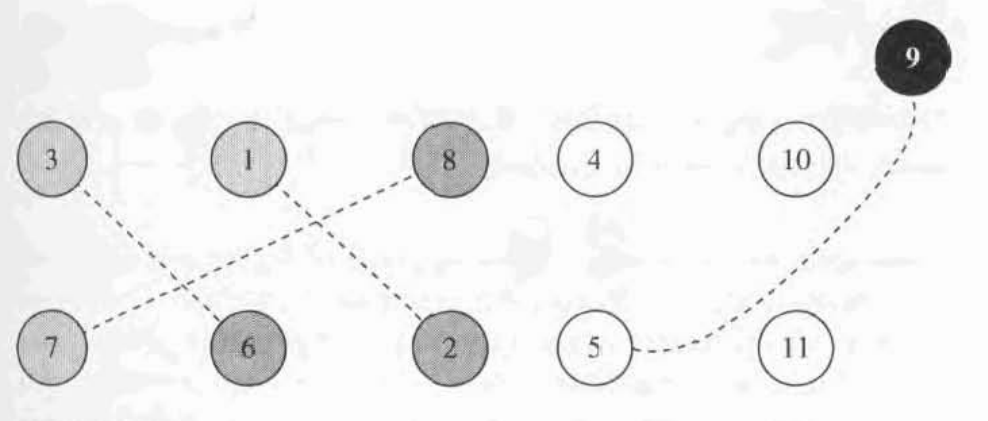
\includegraphics[width=0.5\textwidth]{Conflict_graphs_for_the_mtlltiplier_and_ALU_types}
    \caption{Conflict graphs for the mtlltiplier and ALU types.Conflict graphs for the mtlltiplier and ALU types. \cite{b1}}
    \label{fig:Conflict_graphs_for_the_mtlltiplier_and_ALU_types}
\end{figure}


In some particular cases, it is possible to exploit the structure of the sequencing graph to derive compatibility and conflict graphs with special properties that make the partitioning and coloring tractable. This will be considered in the following section.



\subsection{Conflict graph as an interval for non hierarchical graph}


Let us consider now the conflict graphs for each resource type. The execution intervals for each operation are $ \{[t_{i},t_{i}+d_{i}-1];i=1,2,...,n_{ops}\} $ and the edges of the conflict graphs denote intersections among intervals; hence they are interval graphs. The search for a minimum coloring of an interval graph can be achieved in polynomial time.  Usually, resource Sharing and binding is achieved by considering the conflict graphs for each type, because resources are assumed to have a single type. Thus, the overall conflict graph is of limited interest, even though it can be derived from the conflict graphs of each resource type in a straightforward way.

Consider again the scheduled sequencing graph of Figure \ref{Scheduled_sequencing_graph}, where all operations have unit execution delay. The set of intervals corresponding to the conflict graphs is shown in Figure \ref{Intervals_corresponding_to_the_conflict_grap}. Overlapping intervals correspond to edges in the conflict 
graph for each type. When considering the multiplier, the conflict edges are $ \{v_{1},v_{2}\} $,$ \{v_{3},v_{6}\} $ and $ \{v_{7},v_{8}\} $. When considering the ALU, the conflict edge is $ \{v_{5},v_{9}\} $.


\begin{figure}[h]
    \centering
    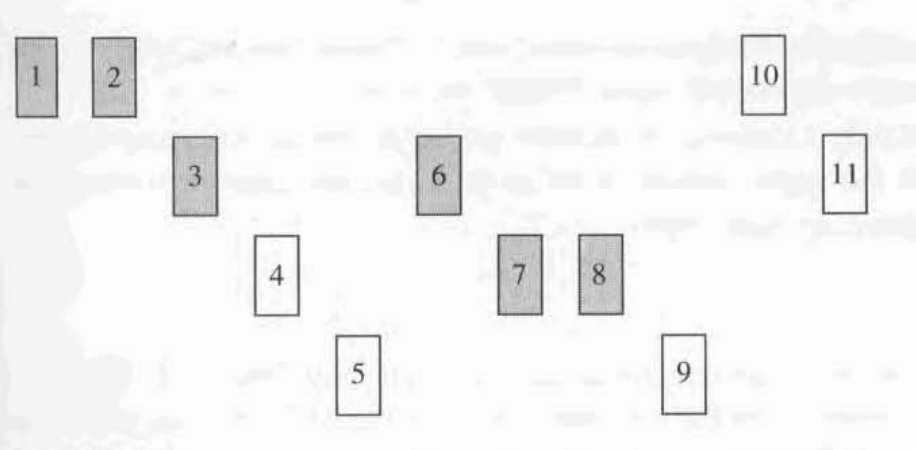
\includegraphics[width=0.5\textwidth]{Intervals_corresponding_to_the_conflict_grap}
    \caption{ Intervals corresponding to the conflict graph \cite{b1}}
    \label{fig:Intervals_corresponding_to_the_conflict_grap}
\end{figure}


\begin{figure}[h]
    \centering
    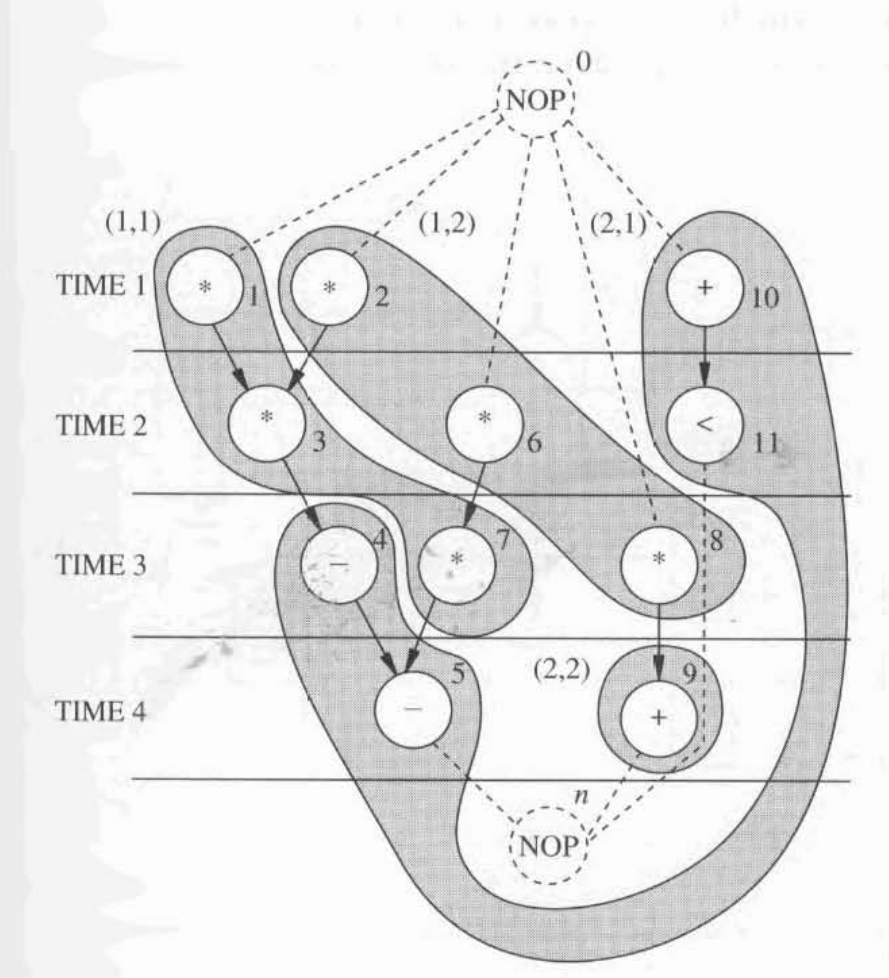
\includegraphics[width=0.5\textwidth]{Scheduled_an_bound_sequencing}
    \caption{ Scheduled and bound sequencing graph \cite{b1}}
    \label{fig:Scheduled_an_bound_sequencing}
\end{figure}

\subsection{Analysis using ILP model}

It is instructive to show that the binding problem can be formulated with an ILP model. For the sake of simplicity, we assume first that all operations and resources have the same type. We use a set of binary decision variables with two indices, $ B=\{b_{ir};i=1,2,...,n_{pos};r=1,2,...,a\} $, and a set of binary decision constants with two indices, $ X=\{x_{il};i=1,2,...,n_{pos};l=1,2,...,\lambda+1\} $, where $ a\leq n_{ops} $ is an upper bound on the number of resources to be used. We use the set notation for the variables in B, rather than a matrix notation, because we do not make use of matrix operations. The binary variable,$ b_{ir} $ is 1 only when operation $ v_{i} $ is bound to resource r, i.e., $ \beta(v_{i})=(1,r) $. The binary constant, $ x_{il} $ is 1 only when operation $ v_{i} $  starts in step 1 of the schedule, i.e., $ l = t{i} $. These values are known constants, because we consider scheduled sequencing graphs. 

Searching for a binding compatible with a given schedule (represented by X) and a resource bound a is equivalent to searching for a set of values of B satisfying 
the following constraints: 

\begin{equation}\label{a}
 \sum_{r=1}^{a} b_{ir} = 1, i=1,2,...,n_{ops} 
\end{equation}

\begin{equation}\label{b}
\sum_{i=1}^{n_{ops}} b_{ir}\sum_{m=l-d_{i}+1}^{l} x_{im} \leq 1, l=1,2,...,\lambda + 1, r=1,2,...,a 
\end{equation}

\begin{equation}\label{c}
b_{ir} \in \{0,1\}, 1 =1,2,...,n_{ops}, r=1,2,...,a
\end{equation}

Constraint \ref{a} states that each operation $ v_{i} $  should be assigned to one and only one resource. Constraint \ref{b} states that at most one operation can be executing, among 
those assigned to resource r, at any time step. Note that it suffices to require the variables in B to he non-negative integers to satisfy \ref{c}. Hence the problem can be formulated as an ILP and not necessarily as a ZOLP. 
This model can be easily extended to include multiple operation types. Nevertheless, the disjointness of the types makes it easier to formulate and solve as many independent binding problems as each type. 

Consider again the scheduled sequencing graph of Figure \ref{Scheduled_sequencing_graph}. The operations have two types (labeled 1 for the multiplier and 2 for the ALU) and unit execution delays. Therefore a feasible binding satisfies the constraints: 

\begin{center}

$ \sum_{r=1}^{a_{1}} b_{ir} = 1,\forall_{i} : \tau(v_{i})=1 $

$ \sum_{i=:\tau(v_{i})=1}^{} b_{ir} x_{il} \leq 1, l=1,2,...,\lambda + 1, r=1,2,...,a_{1}$

$ \sum_{r=1}^{a_{2}} b_{ir} = 1,\forall_{i} : \tau(v_{i})=2$

$ \sum_{i=:\tau(v_{i})=2}^{} b_{ir} x_{il} \leq 1, l=1,2,...,\lambda + 1, r=1,2,...,a_{2}$
\end{center}


The constants in the set X are all zero, except for $ x_{1,1},x_{1,1},x_{2,1},x_{3,2},x_{4,3},x_{5,4},x_{6,2},x_{7,3},x_{8,3},x_{9,4},x_{10,1},x_{11,2} $ which are 1. Then, an implementation with $ a_{1} =1$ multiplier would correspond to finding a 
solution to: 

\begin{center}

$ b_{i1} = 1, \forall_{i} \in \{1,2,3,6,7,8\} $

$ \sum_{i\in \{1,2,3,6,7,8\}}^{} b_{i1} x_{il} \leq 1, l=1,2,...,5$
\end{center}

Such a solution does not exist, because the second constraint would imply $ b_{1,1}=b_{1,2} \leq 1 $, which contradicts the first one. An implementation with $ a_{1} =2$ multipliers would correspond to finding a solution to:

\begin{center}

$ b_{i1}=b_{i2} = 1, \forall_{i} \in \{1,2,3,6,7,8\} $

$ \sum_{i\in \{1,2,3,6,7,8\}}^{} b_{i1} x_{il} \leq 1, l=1,2,...,5$

$ \sum_{i\in \{1,2,3,6,7,8\}}^{} b_{i2} x_{il} \leq 1, l=1,2,...,5$
\end{center} 

which admits the solution $ b_{1,1}=1,b_{2,2}=1,b_{3,1}=1,b_{6,2}=1,b_{7,1}=1,b_{8,2}=1 $, all other elements of B with first subscript $ i \in \{I, 2,3.6,7,8\}$ being zero. The tabulation of the binding is the following, where the binding of the ALUs can be computed in a similar way. The bound sequencing graph is shown in Figure \ref{tabu} . 

\begin{figure}[h]
    \centering
    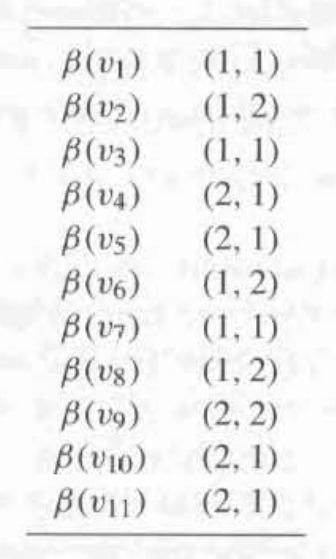
\includegraphics[width=0.18\textwidth]{tabu}
    \caption{ Tne tabulation of the binding \cite{b1}}
    \label{fig:tabu}
\end{figure}

Note that in the particular case of a non-hierarchical graph, solving the ILP problem may he far less efficient than coloring the corresponding interval graph.


\subsection{Resource sharing and binding analysis for non hierarchical graph}

Let us now consider hierarchical sequencing graphs. A simplistic approach to resource sharing is to perform it independently within each sequencing graph entity. Such an approach is overly restrictive, because it would not allow sharing resources in different entities. Therefore we consider here resource sharing across the hierarchy levels. 

Let us first restrict our attention to sequencing graphs where the hierarchy is induced by model calls. When two link vertices corresponding to different called models are not concurrent, any operation pair implementable by resources with the same type and in the different called models is compatible. Conversely, concurrency of the called models does not necessarily imply conflicts of operation pairs in the models themselves.

Consider a model a consisting of two operations: an addition followed by a multiplication. Consider also a model b consisting of two operations: a multiplication followed by an addition. Assume that the addition has l-unit delay and the multiplicalion 2-unit delay. When a model $ m1 $ has a call to model a followed by a call to model b, a and b are not concurrent and the corresponding additions and multiplications are compatible. 
Consider another model $ m2 $ with two calls to a and b that overlap in time, say with start times $ t_{a}=1 $and $ t_{b}=3 $. Then we cannot say a priori that the operations of a and b are conflicting. Indeed the multiplications are not compatible while the additions are! Both situations are shown in \ref{fig:Hierarchical_conflicts_and_compatibility}. 

Therefore the appropriate way of computing the compatibility of operations across different levels of the hierarchy is to flatten the hierarchy. Such an expansion can be done explicitly, by replacing the link vertices by the graphs of the corresponding models, or implicitly, by computing the execution intervals of each operation with respect to the source operation of the rwt model in the hierarchy. 

To determine the properties of the compatibility and conflict graphs, we need to distinguish the cases when models are called once or more than once. In both cases, model calls make the sequencing graph representation modular. In the latter case, model calls express also the sharing of the application-specific resource corresponding to the model. 


\begin{figure}[h]
    \centering
    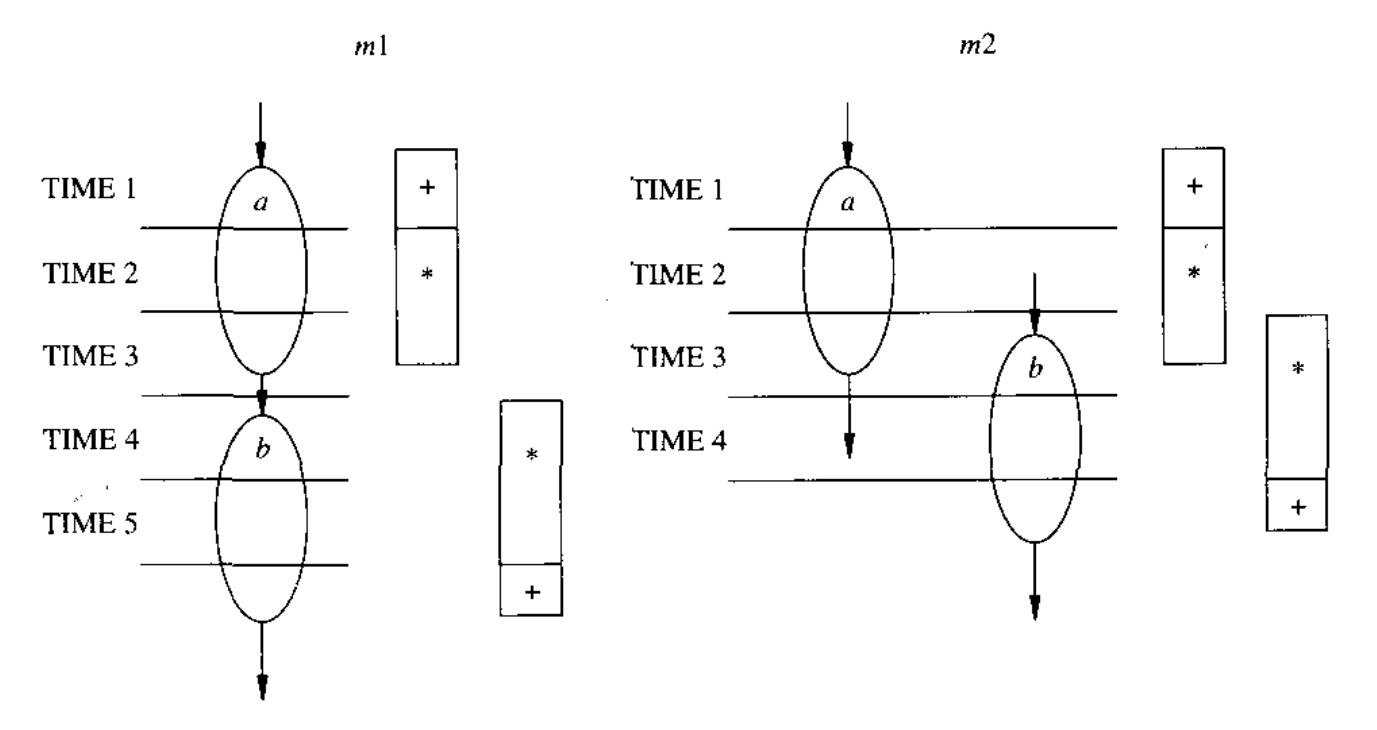
\includegraphics[width=0.5\textwidth]{Hierarchical_conflicts_and_compatibility}
    \caption{ Hierarchical conflicts and compatibility. \cite{b1}}
    \label{fig:Hierarchical_conflicts_and_compatibility}
\end{figure}


When all models are called only once, the hierarchy is only a structured representation of the data-flow information. Thus compatibility and conflict graphs have 
the special properties described in the previous section. 
Let us consider now multiple calls to s model. We question the compatibility 
or conflict of the operations in the called model with those in the calling one, and the 
properties of the corresponding graphs. 


onsider again model a consisting of two operations: an addition followed by a multiplication. By assuming that the addition has 1-unit delay and the multiplication 2-unit delay, model a has an overall delay of 3 units. Consider then model $ m3 $ with two calls to model a that are not concurrent scheduled at times 1 and 5, respectively. Assume also that model $ m3 $ has three other multiplication operations. We question the sharing of the multipliers across the hierarchy. 
A sequencing graph fragment (related to $ m3 $), the execution intervals and the conflict graph for the multiplier type are shown in Figure \ref{fig:Hierarchical_conflicts}. Note that the double call to a results in two non-contiguous execution intervals for the multiplication in a. As a result, the conflict graph is not an intersection among intervals and therefore not an interval graph. It is not even a chordal graph, as shown in Figure \ref{fig:Hierarchical_conflicts} (c).

hereas the computation of the compatibility and conflict graphs is still straightforward, the resulting graphs may no longer have special properties. Therefore their clique partitioning and vertex coloring are now intractable problems. 

\begin{figure}[h]
    \centering
    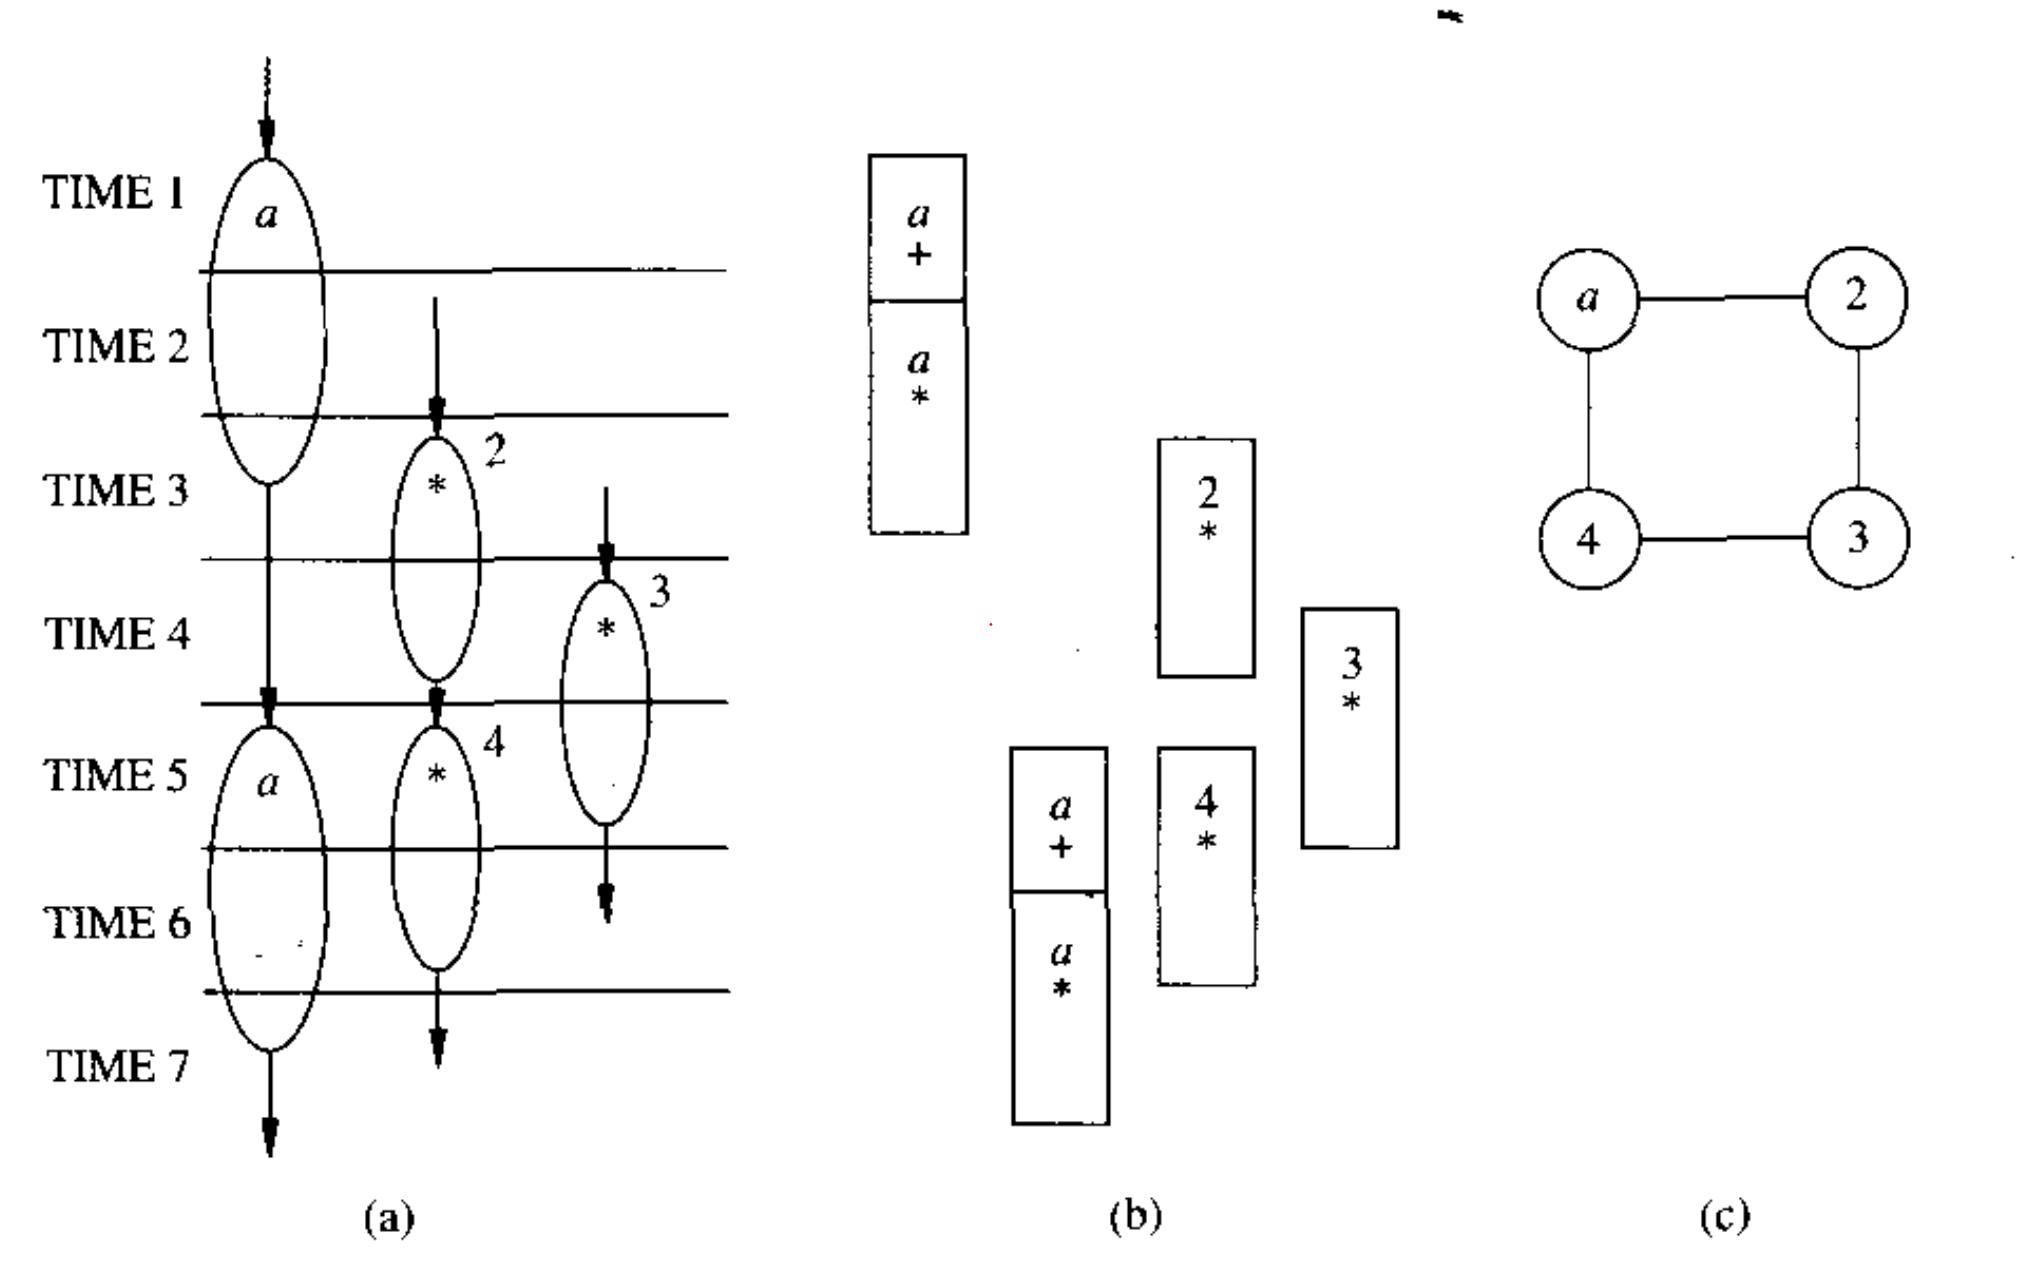
\includegraphics[width=0.5\textwidth]{Hierarchical_conflicts}
    \caption{Hierarchical conflicts. (a) Sequencing graph fragment. (b) Execution intervals. (c) Non-chordal conflict graph. \cite{b1}}
    \label{fig:Hierarchical_conflicts}
\end{figure}


The compatibility of the operations across the hierarchy can be computed in a similar way in the presence of iterative constructs that can be unrolled. Note that a resource bound to one operation in a loop corresponds to a resource bound to multiple instances of that operation when the loop is unrolled. Moreover, that resource may be bound to other operations outside the loop model. Note also that a single model call inside a loop body becomes a multiple call when the loop body is unrolled. Let us consider now branching constructs. When considering operation pairs in two alternative branching bodies, their compatibility corresponds to having the same type. The computation of the compatibility and conflict graphs can still be done by traversing the hierarchy and using Definitions  resource compatibility graph and resource conact graph. The resulting compatibility and conflict graphs may not have any special property, as shown by the following example. 

Consider the sequencing graph of Figure \ref{fig:Conditional_execution} (a). We assume that all operations take 2 time units to execute and that the start times are the following: 
$ t_{a}=1;t_{b}=3;t_{c}=t{d}=2 $. The intervals are shown in Figure \ref{fig:Conditional_execution} (b) and the conflict graph in Figure \ref{fig:Conditional_execution}(c). Note that the alternative nature of operations c and d makes them compatible and prevents a chord $ \{v_{c},v_{d}\} $to be present in the conflict graph. Hence the conflict graph is not an interval gtaph. 


\begin{figure}[h]
    \centering
    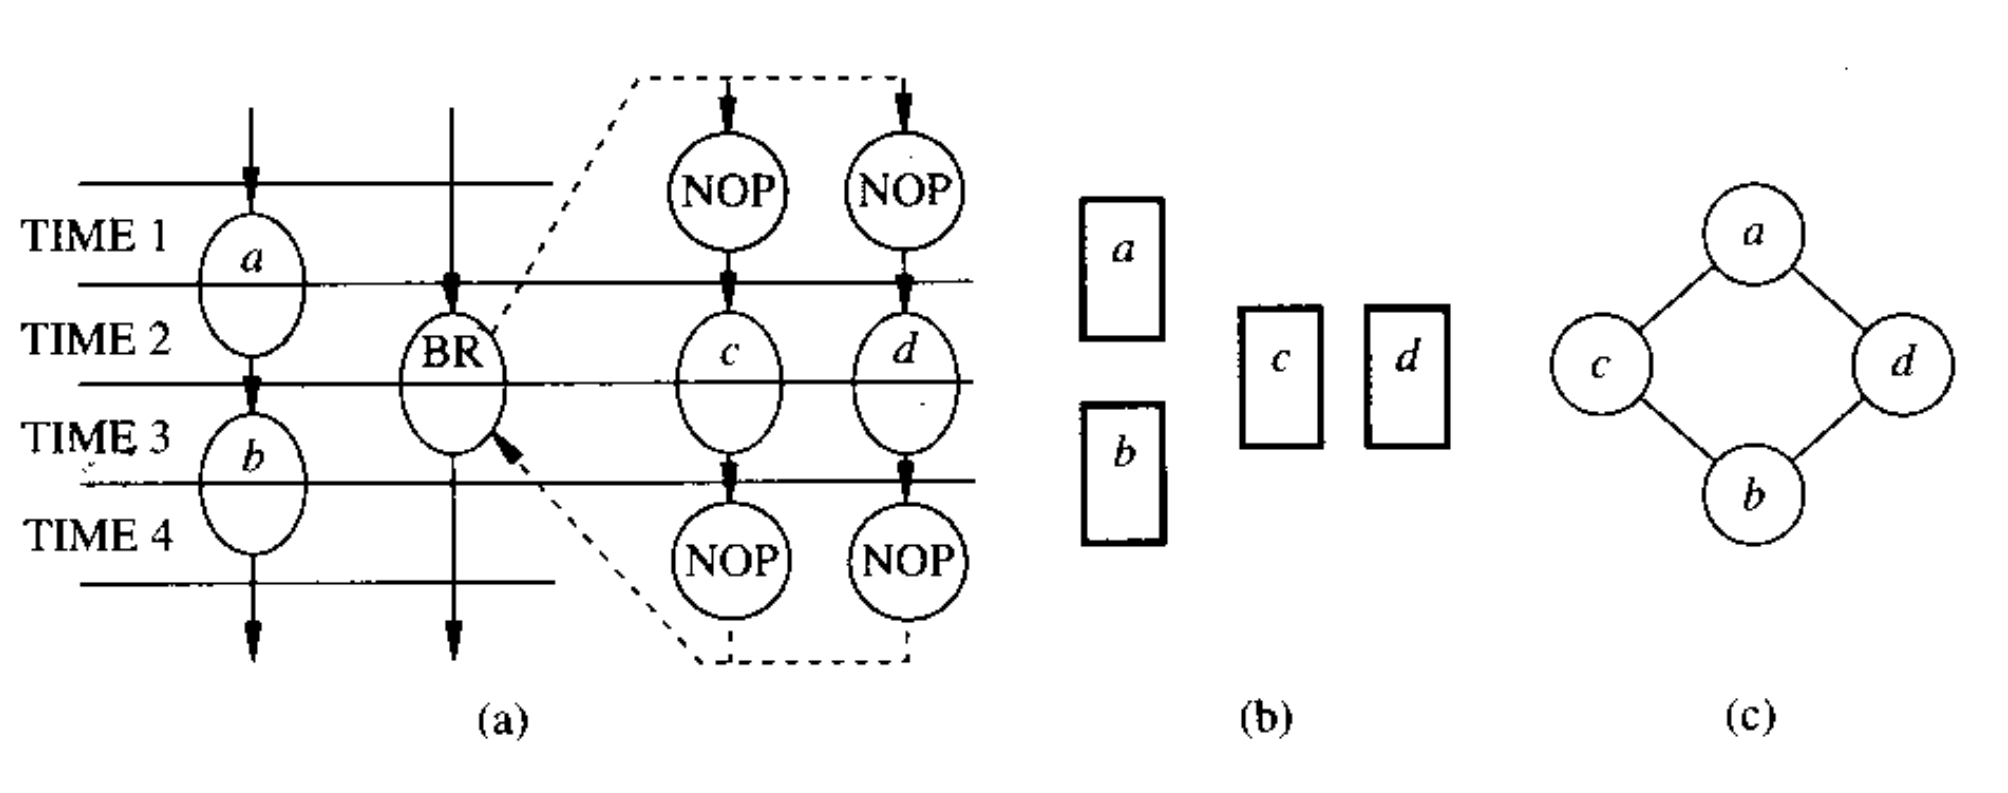
\includegraphics[width=0.5\textwidth]{Conditional_execution}
    \caption{ Conditional execution. (a) Sequencing graph fragment. (b) Execution intervals. (c) Non-chordal conflict graph \cite{b1}}
    \label{fig:Conditional_execution}
\end{figure}